\subsection{Precessão do Giroscópio}

O último experimento sobre esse tópico que vamos realizar é sobre giroscópios, mais precisamente o fenômeno da precessão que eles realizam, que consiste no movimento circular realizado em torno de um ponto de pivô por um objeto que gira, como pode ser visto nas figuras abaixo:

\begin{figure}[H]
  \centering
    \begin{subfigure}[b]{0.48\textwidth}
        \centering
        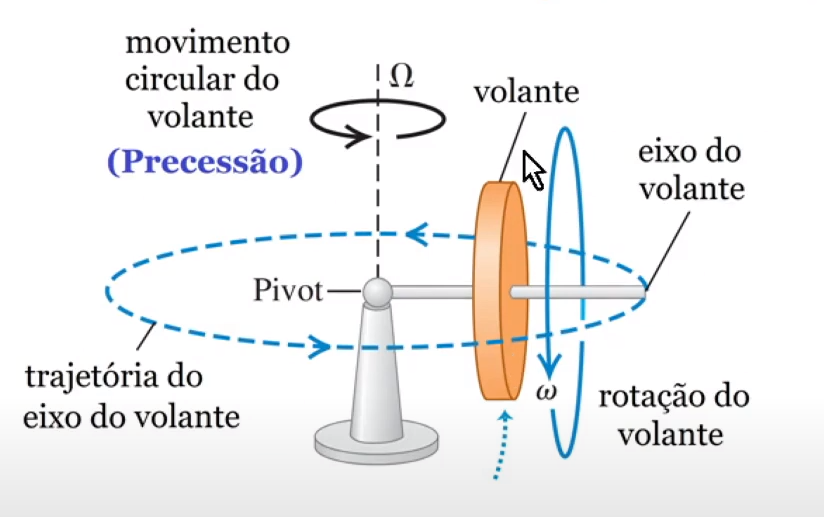
\includegraphics[width=\textwidth]{images/movimento-giroscopio.png}
        \caption{Diagrama do movimento de precessão de um giroscópio}
    \end{subfigure}
    \hfill
    \begin{subfigure}[b]{0.48\textwidth}
        \centering
        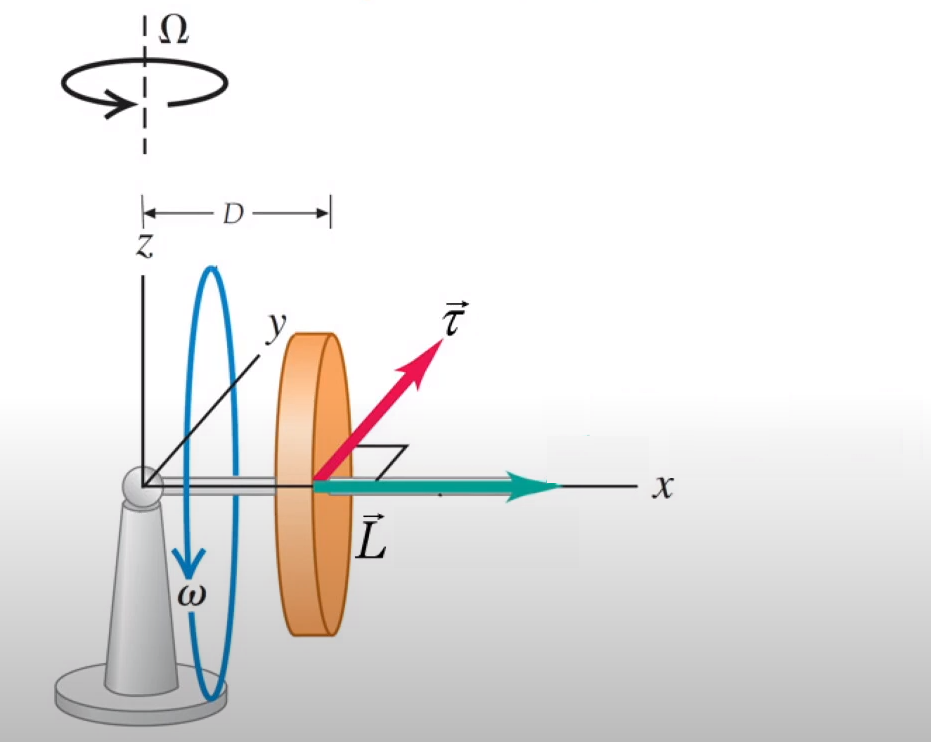
\includegraphics[width=\textwidth]{images/propriedades-giroscopio.png}
        \caption{Vetores que agem sobre o giroscópio}
    \end{subfigure}
\end{figure}

A partir dos diagramas acima, podemos realizar uma série de substituições de equações utilizando as equações básicas de rotação - como foi mostrado no vídeo dessa prática - para encontrar que a frequência da precessão $\Omega _E$ de um giroscópio pode ser estimada pela seguinte equação:

\[ \Omega _{Ei} = \frac{MgD}{I \omega _i} \]

Só que como vamos fazer 4 medidas, para podermos ter um resultado mais confiável, a frequência que utilizaremos será a média aritmética desses valores, e a incerteza dessa medida será dada pelo desvio padrão:

\[ \overline{\Omega _E} = \frac{\sum_{i=1}^{4} \Omega _{Ei}}{4}\]
\[ \Delta \overline{\Omega _E} = \sqrt{\frac{\sum_{i=1}^{4} (\Omega _i - \overline{\Omega _E})^2}{4}}\]

% \[ N = MgD \]
% \[ D = I \omega \]
% \[ \Omega _e = \frac{N}{D} \]

% E as incertezas dessa medida se dão por:

% \[ \Delta N = g \cdot (M \cdot \Delta D + \Delta M \cdot D) \]
% \[ \Delta D = \Delta I \cdot \omega + I \cdot \Delta \omega \]
% \[ \Delta \Omega _e = g \cdot \frac{(\Delta N \cdot D) + (N \cdot \Delta D)}{D^2} \]

Detalhe que para determinar \textit{I} haverá uma diferença nesse caso do giroscópio, pois diferente do Disco de Maxwell (tópico 2.1), não será possível desmontar a peça para pesar cada componente individualmente. Precisaremos calcular a massa da forma indireta, utilizando o valor da densidade do material que ela é feita.\\

\begin{figure}[H]
  \centering
  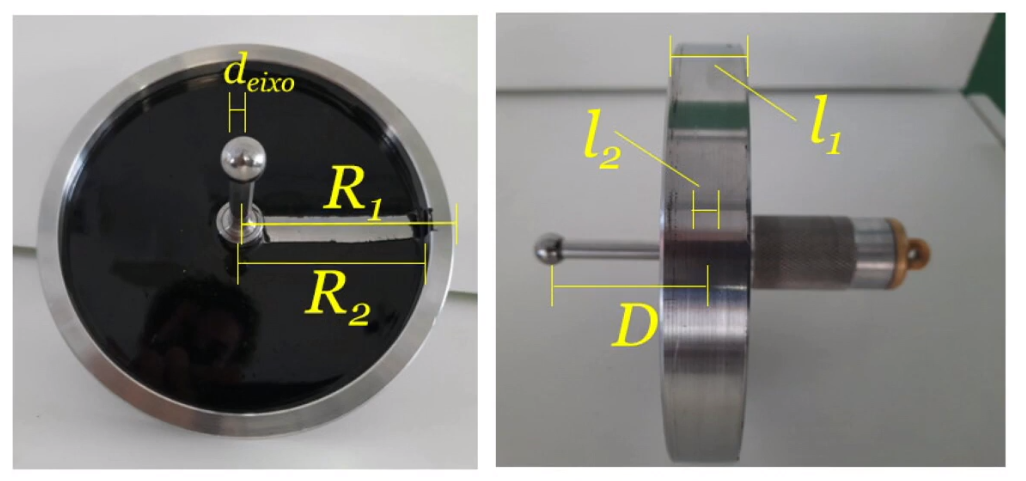
\includegraphics[scale=0.5]{images/medidas-giroscopio.png}
  \caption{Dimensões do giroscópio a serem consideradas.}
\end{figure}

Considerando as dimensões acima, teremos que a massa de cada componente (eixo, disco e anel) pode ser calculada pelo volume vezes a densidade do material - que no caso será aço. As formulas então serão:

\[ r_{eixo} = \frac{d_{eixo}}{2} \Rightarrow m_e = (2 D \pi r_{eixo}^2) \cdot \rho_{aco}\]

\[ m_d = (l_2 \pi R_2^2) \cdot \rho_{aco} \]

\[ m_a = (l_1 \pi R_1^2) \cdot \rho_{aco} \]

E propagando as incertezas:

\[ \Delta r_{eixo} = \frac{\Delta d_{eixo}}{2} \Rightarrow \Delta m_e = \rho_{aco} \cdot 2 \pi \left( \Delta D \cdot r_{eixo}^2 + D \cdot 2 \cdot r_{eixo} \cdot \Delta r_{eixo} \right)\]

\[ \Delta m_d = \rho_{aco} \cdot \pi \left( \Delta l_2 \cdot R_2^2 + l_2 \cdot 2 \cdot R_2 \cdot \Delta R_2 \right) \]

\[ \Delta m_a = \rho_{aco} \cdot \pi \left( \Delta l_1 \cdot R_1^2 + l_1 \cdot 2 \cdot R_1 \cdot \Delta R_1 \right) \]

Após os cálculos das massas, podemos estimar os momentos de inércia da mesma forma que na Roda de Maxwell, as fórmulas serão as mesmas para cada componente).\\

Agora, como forma de comparação se soubermos o tempo que o giroscópio demora para fazer uma volta podemos calcular diretamente qual é a frequência de rotação $\Omega _d$. Esse valor pode ser obtido pela simples relação de em quanto tempo $t_i$ o giroscópio efetuará uma 3 voltas completas:

\[\Omega _D = \frac{3 \cdot (2 \pi)}{t _i} = \frac{6\pi}{t _i}\]

Da mesma forma que o anterior, utilizaremos a média ponderada dos 4 valores e contrado e propagando as incertezas pelo desvio padrão para essa medida, teremos:

\[ \overline{\Omega _D} = \frac{\sum_{i=1}^{4} \Omega _{Di}}{4}\]

\[ \Delta \overline{\Omega _D} = \sqrt{\frac{\sum_{i=1}^{4} (\Omega _{Di} - \overline{\Omega _D})^2}{4}}\]
